\documentclass[xcolor=svgnames]{beamer} 
\usefonttheme[onlymath]{serif}
\usepackage{tcolorbox}
\usepackage{multimedia}
\usepackage[utf8]{inputenc}
\usepackage[T1]{fontenc}
\usepackage[spanish]{babel}
\usepackage{mathtools}  % amsmath improved
%\usepackage{amsmath}
\usepackage{amssymb}
\usepackage{amsthm}
\usepackage{cancel}
\usepackage{multimedia}
\usepackage{algorithm2e}
%\usepackage{algorithm}
%\usepackage{algorithmic}
\usepackage{xcolor}
%\usepackage{pgfplots}
\usepackage{booktabs}   % Fancy table borders.

\newcommand{\grn}[1]{\textcolor{Green}{#1}}
\newcommand{\red}[1]{\textcolor{Red}{#1}}
\newcommand{\ple}[1]{\textcolor{Purple}{#1}}
\newcommand{\ong}[1]{\textcolor{DarkGoldenrod}{#1}}

%~~~~~~~~~~~~~~~~~~~~~~~~~~~~~~~~~~~~~~~~~~~~~~~~~~~~~~~~~~~~~~~~~~~~~~~~~~
%                         Beamer theme and colors

\usetheme{Warsaw}
%9 77 141

\definecolor{eafitColor}{rgb}{0.03515625,0.30078125,0.55078125}
\definecolor{eafitColor2}{rgb}{ 0.30859375,  0.5234375 ,  0.6953125}
\definecolor{mygreen}{rgb}{0.0 ,0.6, 0.0}


\usecolortheme[named=eafitColor]{structure} 
\setbeamercolor*{palette primary}{use=structure,fg=white,bg=eafitColor}
\setbeamercolor*{palette quaternary}{fg=white,bg=eafitColor2!90!eafitColor2}

%~~~~~~~~~~~~~~~~~~~~~~~~~~~~~~~~~~~~~~~~~~~~~~~~~~~~~~~~~~~~~~~~~~~~~~~~~~
%                    Put the page number on the slide

\defbeamertemplate*{footline}{shadow theme}
{%
  \leavevmode%
  \hbox{\begin{beamercolorbox}[wd=.5\paperwidth,ht=2.5ex,dp=1.125ex,leftskip=.3cm plus1fil,rightskip=.3cm]{author in head/foot}%
    \usebeamerfont{author in head/foot}\hfill\insertshortauthor
  \end{beamercolorbox}%
  \begin{beamercolorbox}[wd=.5\paperwidth,ht=2.5ex,dp=1.125ex,leftskip=.3cm,rightskip=.3cm plus1fil]{title in head/foot}%
    %\usebeamerfont{title in head/foot}\insertshorttitle\hfill\insertframenumber\,/\,\inserttotalframenumber%
    \usebeamerfont{title in head/foot}\insertshorttitle\hfill\insertframenumber\,/\,\inserttotalframenumber%
  \end{beamercolorbox}}%
  \vskip0pt%
}
%\setbeamertemplate{footline}{\hfill\insertframenumber/\inserttotalframenumber} 


%~~~~~~~~~~~~~~~~~~~~~~~~~~~~~~~~~~~~~~~~~~~~~~~~~~~~~~~~~~~~~~~~~~~~~~~~~~
%                             Color equations

\everymath{\color{blue}}
\everydisplay{\color{blue}}


\newcommand{\highlight}[1]{%
  \colorbox{yellow!50}{$\displaystyle#1$}}
  
\newcommand{\mathColor}[1]{{\color{blue}#1}}
\newcommand{\emphRed}[1]{{\color{red}#1}}

%~~~~~~~~~~~~~~~~~~~~~~~~~~~~~~~~~~~~~~~~~~~~~~~~~~~~~~~~~~~~~~~~~~~~~~~~~~
%                           Example environment

 \newtheoremstyle{example}{\topsep}{\topsep}%
     {}%         Body font
     {}%         Indent amount (empty = no indent, \parindent = para indent)
     {\bfseries}% Thm head font
     {}%        Punctuation after thm head
     {\newline}%     Space after thm head (\newline = linebreak)
     {\thmname{#1}\thmnumber{ #2}\thmnote{ #3}}%         Thm head spec

   \theoremstyle{example}
%   \newtheorem{example}{Example}[chapter]

%~~~~~~~~~~~~~~~~~~~~~~~~~~~~~~~~~~~~~~~~~~~~~~~~~~~~~~~~~~~~~~~~~~~~~~~~~~
%                           Vectors and Tensors

\if@mathematic
   \def\vec#1{\ensuremath{\mathchoice
                     {\mbox{\boldmath$\displaystyle\mathbf{#1}$}}
                     {\mbox{\boldmath$\textstyle\mathbf{#1}$}}
                     {\mbox{\boldmath$\scriptstyle\mathbf{#1}$}}
                     {\mbox{\boldmath$\scriptscriptstyle\mathbf{#1}$}}}}
\else
   \def\vec#1{\ensuremath{\mathchoice
                     {\mbox{\boldmath$\displaystyle#1$}}
                     {\mbox{\boldmath$\textstyle#1$}}
                     {\mbox{\boldmath$\scriptstyle#1$}}
                     {\mbox{\boldmath$\scriptscriptstyle#1$}}}}
\fi


\def\Real{\mathbb{R}}%
\newcommand{\mvM}{\text{max }\sigma_\text{vm} (\bs)}
\newcommand{\D}{\displaystyle}
\newcommand{\bm}[1]{\mbox{\boldmath$#1$}}

\def\bN{\bm{N}}
\def\bell{\boldsymbol \ell}%
\newcommand{\balpha}{\bm{\alpha}}
\def\bomega{\boldsymbol{\omega}}
\def\bsigma{\boldsymbol{\sigma}}
\DeclareMathOperator{\Div}{div}

\def\<{\left<}
\def\>{\right>}


% If you want to put an aditional slide with the section name at the beginning of 
% each section uncomment this two lines

\AtBeginSection{\frame{\sectionpage}}
\AtBeginSubsection{\frame{\subsectionpage}}

%~~~~~~~~~~~~~~~~~~~~~~~~~~~~~~~~~~~~~~~~~~~~~~~~~~~~~~~~~~~~~~~~~~~~~~~~~~~~~~~

\graphicspath{{../imagenes/},{figures2/}}

%\logo{Mecánica Aplicada\includegraphics[width=1.5cm]{logoEAFIT}\hspace{.5cm}} 
\logo{
\includegraphics[width=1.5cm]{Logotipo EAFIT azul en PNG.png}\vspace{-.2cm}} 
%  look later for this (manuel)
%http://tex.stackexchange.com/questions/27906/positioning-logo-in-the-front-page-as-well-as-slides


\title[Programación de Computadores]{ST0240-063 }
\author{Sergio Andrés Monsalve Castañeda \\ \textless smonsal3@eafit.edu.co\textgreater \newline \newline Juan F. Cardona Mc'Cormick \\ \textless fcardona@eafit.edu.co\textgreater}
\institute{
  Departamento de Informática y Sistemas \\
  Universidad EAFIT, Medellin, Colombia\\\vspace{0.5cm}
  \scalebox{2}{\insertlogo}\\\vspace{1cm}
}
%\date{September 13, 2015}
\date{Julio, 2016}

\makeatletter
    \newenvironment{withoutheadline}{
        \setbeamertemplate{headline}[default]
        \def\beamer@entrycode{\vspace*{-\headheight}}
    }{}
\makeatother

%~~~~~~~~~~~~~~~~~~~~~~~~~~~~~~~~~~~~~~~~~~~~~~~~~~~~~~~~~~~~~~~~~~~~~~~~~~
% Comment this line to remore the table of contents on top of the slide

%\setbeamertemplate{headline}{}

\beamertemplatenavigationsymbolsempty
%~~~~~~~~~~~~~~~~~~~~~~~~~~~~~~~~~~~~~~~~~~~~~~~~~~~~~~~~~~~~~~~~~~~~~~~~~~

\begin{document}

\setbeamertemplate{background canvas}{
%	    \includegraphics[width=1.1\textwidth]{region}
}
	
\begin{frame}[plain]
	\titlepage
\end{frame}
\setbeamertemplate{background canvas}{}

%\maketitle 

%~~~~~~~~~~~~~~~~~~~~~~~~~~~~~~~~~~~~~~~~~~~~~~~~~~~~~~~~~~~~~~~~~~~~~~~~~~

 %\section*{Outline}
\begin{withoutheadline}
  \begin{frame}
    \setcounter{tocdepth}{1}
    \frametitle{Outline}     
    \tableofcontents
  \end{frame}
\end{withoutheadline}

\begin{frame}
  \frametitle{Programa}
  \begin{block}{Capítulo 1. Conceptos básicos de los sistemas operativos.}
    \begin{itemize}%[<+->]
    \item Definición de un sistema operativo.
      % \item Historia de los sistemas operativos.
    \item Componentes de los sistemas operativos (introducción).
    \item Procesos.
    \item Administración de memoria.
    \item Administración de recursos y planificación.
    \item Componentes de los sistemas operativos (detallado).
    \item Características de los sistemas operativos modernos.
    \item El mundo según C.
    \end{itemize}
  \end{block}
\end{frame}


\begin{frame}
  \frametitle{Programa}
  % \begin{beamercolorbox}[wd=\textwidth,rounded=false,shadow=true]
  %   {block body example}
  \begin{block}{Capítulo 2. Proceso e hilos.}
    \begin{itemize}%[<+->]
    \item Proceso.
    \item Multitarea.
    \item Información del proceso.
    \item Estados del proceso.
    \item Hilos.
    \item Multiprocesamiento simétrico.
    \item Microkernel.
    \item Planificación de la CPU.
    \item Ejemplos de planificación en Windows y Linux.
    \end{itemize}
    % \end{beamercolorbox}
  \end{block}
\end{frame}

\begin{frame}[shrink]
  \frametitle{Programa}
  \begin{block}{Capítulo 3. Comunicación, concurrencia y bloqueos.}
    \begin{itemize}%[<+->]
    \item Principios de concurrencia.
    \item El problema de la sección crítica.
    \item Solución por software.
    \item Solución por hardware.
    \item Semáforos.
    \item Secciones críticas.
    \item Monitores.
    \item Paso de mensajes.
    \item Transacciones atómicas.
    \item Problemas clásicos de la concurrencia.
    \item Ejemplo de semáforos, monitores, paso de mensajes en
      Windows y Linux.
    \end{itemize}
  \end{block}
\end{frame}

\begin{frame}
  \frametitle{Programa}
  \begin{block}{Capítulo 3. Comunicación, concurrencia y bloqueos. \tiny{(continuación).}}
    \begin{itemize}%[<+->]
    \item Modelo del sistema de bloqueos mutuos.
    \item Caracterización de bloqueos mutuos.
    \item Métodos para manejar bloqueos mutuos.
    \item Prevención de bloqueos mutuos.
    \item Evitar bloqueos mutuos.
    \item Detección de bloqueos mutuos.
    \item Recuperación de bloqueos mutuos.
    \item Recuperación después de un bloqueo mutuo.
    \item Estrategia combinada para el manejo de bloqueos mutuos.
    \end{itemize}
  \end{block}
\end{frame}

\begin{frame}[shrink]
  \frametitle{Programa}
  \begin{block}{Capítulo 4. Gestión de memoria.}
    \begin{itemize}%%[<+->]
    \item Antecedentes.
    \item Requerimientos de gestión de memoria.
    \item Espacio de direcciones lógico y físico.
    \item Intercambio.
    \item Asignación continua.
    \item Paginación.
    \item Segmentación.
    \item Segmentación con paginación.
    \item Memoria virtual.
    \item Paginación por demanda.
    \item Desempeño de la paginación por demanada.
    \item Reemplazo de páginas.
    \item Algoritmo de reemplazo de páginas.
    \item Asignación de marcos.
    \item Hiper--paginación.
    \item Segmentación por demanda.
    \item Gestión de memoria en Linux y Windows.
    \end{itemize}
  \end{block}
\end{frame}


\begin{frame}
  \frametitle{Programa}
  \begin{block}{Capítulo 5. Entrada y salida.}
    \begin{itemize}%[<+->]
    \item Generalidades.
    \item Hardware de E/S (conexión, dispositivos, arquitectura del
      sistema).
    \item Interfaz de E/S.
    \item Almacenamiento secundario.
    \item Almacenamiento terciario.
    \item El reloj.
    \item La terminal.
    \item Manejo de E/S en Windows y Linux.
    \end{itemize}
  \end{block}
\end{frame}

\begin{frame}
  \frametitle{Programa}
  \begin{block}{Capítulo 6. Gestión de ficheros y directorios.}
    \begin{itemize}%[<+->]
    \item El concepto de fichero.
    \item Métodos de acceso.
    \item Estructura de directorios.
    \item Protección.
    \item Semántica de consistencia.
    \item Estructura de sistema de ficheros.
    \item Métodos de asignación.
    \item Eficiencia y desempeño.
    \item Recuperación.
    \item Gestión de ficheros en Linux y Windows.
    \end{itemize}
  \end{block}
\end{frame}

\begin{frame}[shrink]
  \frametitle{Programa}
  \begin{block}{Capítulo 7. Seguridad y protección. Opcional.}
    \begin{itemize}%[<+->]
    \item Amenazas de seguridad.
    \item Protección.
    \item Intrusos.
    \item Software malicioso.
    \item Objetivos de protección.
    \item Matriz de acceso.
    \item Implementación de la matriz de acceso.
    \item Sistemas basado en capacidades.
    \item Protección basada en el lenguaje.
    \item Diseño de sistemas operativos seguros.
    \item Criptografía.
    \item Seguridad y protección de sistemas operativos de propósito general.
    \item Servicios de protección de seguridad.
    \item Clasificación de seguridad de los computadores.
    \item Seguridad en Linux y Windows.
    \end{itemize}    
  \end{block}
\end{frame}

\section{Docente}

\begin{frame}
  \frametitle{Docente}
  \begin{beamercolorbox}[wd=\textwidth,rounded=false,shadow=true]
    {block body example}
    \begin{quote}
      Sergio Andrés Monsalve Castañeda
      \\
      Oficina: Bloque 19 - 4 piso - 408.
      \\
      % Horario: Lunes (14:00 - 15:00), Martes y Jueves (11:00 - 12:00),
      % \\
      % Viernes: (17:00 - 18:00).
      % \\
      Correo: smonsal3@eafit.edu.co
      %% \\
      %% Chat: fcardona@eafit.edu.co
      %% \\
      %% Twitter: @fcardonaeafit
    \end{quote}
  \end{beamercolorbox}
\end{frame}

\section{Libro guía}

\begin{frame}
  \frametitle{Libro guía}
  \begin{columns}
    \begin{column}{0.5\textwidth}
      Sistemas Operativos Modernos
      \\
      Tercera Edición.
      \\
      Andrew S. Tanenbaum -- Herbert Bos
      \\
      Editorial. Pearson.
    \end{column}
    \begin{column}{0.5\textwidth}

    \end{column}
  \end{columns}
\end{frame}

\section{Evaluación}

\begin{frame}
  \frametitle{Evaluación}
  \begin{itemize}%%[<+->]
  \item Taller 1 (5\%) - Semana 2  (2016-08-17)
  \item Taller 2 (5\%) - Semana 4  (2016-08-17)
  \item Taller 3 (10\%) - Semana 6  (2016-08-17)
  \item Taller 1 (10\%) - Semana 8  (2016-08-17)
  \item Taller 2 (10\%) - Semana 10  (2016-08-17)
  \item Seguimiento (10\%) 
  \item Práctica 1 (15\%) - Semana 11 (2016-09-19)
  \item Práctica 2 (15\%) - Semana 13 (2016-10-26)
  \item Práctica Final (20\%)
  \end{itemize}
\end{frame}


%--------------------------------------------------------------------------
% \section{Módulo 0 -- Clase Número 1}

% \subsection{Presentación del Curso}
% \begin{frame}
% \frametitle{Juan David Pineda--Cárdenas}
% \begin{columns}
%   \begin{column}[ht]{5cm}
%     Ingeniero de Sistemas Egresado de la Universidad EAFIT, Medellín, Colombia. Candidato a Magister en Seguridad de la Información en la Universidad Oberta de Catalunya, España. Actualmente se desempeña como coordinador técnico del Centro de Computación Científica APOLO, en la Universidad EAFIT.
%   \end{column}
%   \begin{column}[ht]{5cm}
%     \begin{figure}[ht]
%       \centering
%       \includegraphics[scale=0.06]{../imagenes/juanpineda.png}
%       \caption{<jpineda2@eafit.edu.co>}
%     \end{figure}
%   \end{column}
% \end{columns}
% \end{frame}

% \begin{frame}
% \frametitle{Temas de Interés}
% \begin{columns}
%   \begin{column}[ht]{5cm}
%     \begin{itemize}
%       \item Computación de Alto Rendimiento
%       \item Seguridad de la Información
%       \item Criptomonedas  
%       \item Sistemas Embebidos
%       \item IoT
%     \end{itemize}
%   \end{column}
%   \begin{column}[ht]{5cm}
%     \begin{figure}[ht]
%       \centering
%       \includegraphics[scale=0.1]{../imagenes/failure.png}
%       \caption{Matrix}
%     \end{figure}
%   \end{column}
% \end{columns}
% \end{frame}


% \begin{frame}
% \frametitle{Objetivos}
% \begin{enumerate}
% \item Entender, manejar y utilizar los conceptos básicos de la programación \textbf{imperativa}.
% \item Diseñar soluciones de software para la resolución de problemas simples de programación, a través del desarrollo de programas \textit{top--down}.
% \item Tener un conocimiento básico para desarrollar y diseñar soluciones de programación en los lenguajes de programación VBA para Excel y Matlab.
% \end{enumerate}
% \end{frame}

% \begin{frame}
% \frametitle{Contenido del Curso}
% \begin{enumerate}
% \item \textbf{Módulo 0:} Introducción al curso (3 horas)
% \item \textbf{Módulo 1:} Solución de problemas utilizando el computador (15 horas presenciales)
% \item \textbf{Módulo 2:} Implementación de problemas en VBA (15 horas presenciales)
% \item \textbf{Módulo 3:} Implementación de problemas en MATLAB (15 horas presenciales)
% \end{enumerate}
% \end{frame}

% \begin{frame}
% \frametitle{Evaluación}
% \begin{itemize}
% \item \textbf{Parcial 1:} \alert{(20\%)} Agosto 16. Módulo 1. 
% \item \textbf{Parcial 2:} \alert{(20\%)} Septiembre 20. Módulo 2.
% \item \textbf{Exámenes cortos y tareas:} \alert{(20\%)} A lo largo del Semestre.
% \item \textbf{Práctica VBA:} \alert{(10\%)} Entrega: Septiembre 20. Tres semanas para el desarrollo.
% \item \textbf{Práctica MATLAB:} \alert{(10\%)} Entrega: Noviembre 8. Tres semanas para el desarrollo.
% \item \textbf{Parcial Final:} \alert{(20\%)} Noviembre 1. Módulo 1, 2 y 3. 
% \end{itemize}
% \end{frame}

% \begin{frame}
%   \frametitle{Criterios de Evaluación}
%   \begin{itemize}
%   \item Cumplimiento de los compromisos y fechas acordadas para presentación de trabajos.
%   \item Calidad de las tareas, talleres y prácticas presentadas.
%   \item Apropiación de los conceptos y su importancia en la formación como profesional.
%   \end{itemize}
% \end{frame}

% \begin{frame}
% \frametitle{Evaluación de Exámenes cortos y tareas}
% \begin{itemize}
% \item \textbf{Quiz 1:} \alert{(4\%)}
% \item \textbf{Quiz 2:} \alert{(4\%)}
% \item \textbf{Quiz 3:} \alert{(4\%)}
% \item \textbf{Tarea con Entrega:} \alert{(8\%)}
% \end{itemize}
% \end{frame}

% \begin{frame}
% \frametitle{Políticas dentro de la clase}
% \begin{itemize}
% \item Nada de dispositivos móviles durante la clase.
% \item Nada de páginas no concernientes a la clase.
% \item Ir a clase es un derecho, no un deber.
% \item Los exámenes cortos se anuncian con una semana de antelación.
% \item Si falta a cualquier examen debe presentar supletorio y excusa médica.
% \item En caso de estar en deporte representativo debe avisar con antelación.
% \item \alert{\textbf{Política de 0 tolerancia con fraude.}} Se anuncia a decanatura y pasa a consejo disciplinario.
% \item El nivel del curso es introductorio.
% \item Solo se reciben tareas y mensajes por medio de EAFIT Interactiva.
% \end{itemize}
% \end{frame}

% \begin{frame}
% \frametitle{Políticas dentro de la clase}
% \begin{itemize}
% \item El conducto regular es el Siguiente
%   \begin{itemize}
%     \item \textbf{Profesor:} Juan David Pineda C. <jpineda2@eafit.edu.co>
%     \item \textbf{Coordinadora:} Elizabeth Suescún <esuescu1@eafit.edu.co>
%     \item \textbf{Jefe de Carrera:} Edwin Montoya <emontoya@eafit.edu.co> 
%   \end{itemize}
% \end{itemize}
% \end{frame}

% \begin{frame}
% \frametitle{Libro Guía}
% \begin{columns}
%   \begin{column}[ht]{5cm}
%     Farrell, Joyce. Introducción a la programación lógica y diseño. 7a. Ed. México. Cengage Learning. 2013.
%   \end{column}
%   \begin{column}[ht]{5cm}
%     \begin{figure}[ht]
%       \centering
%       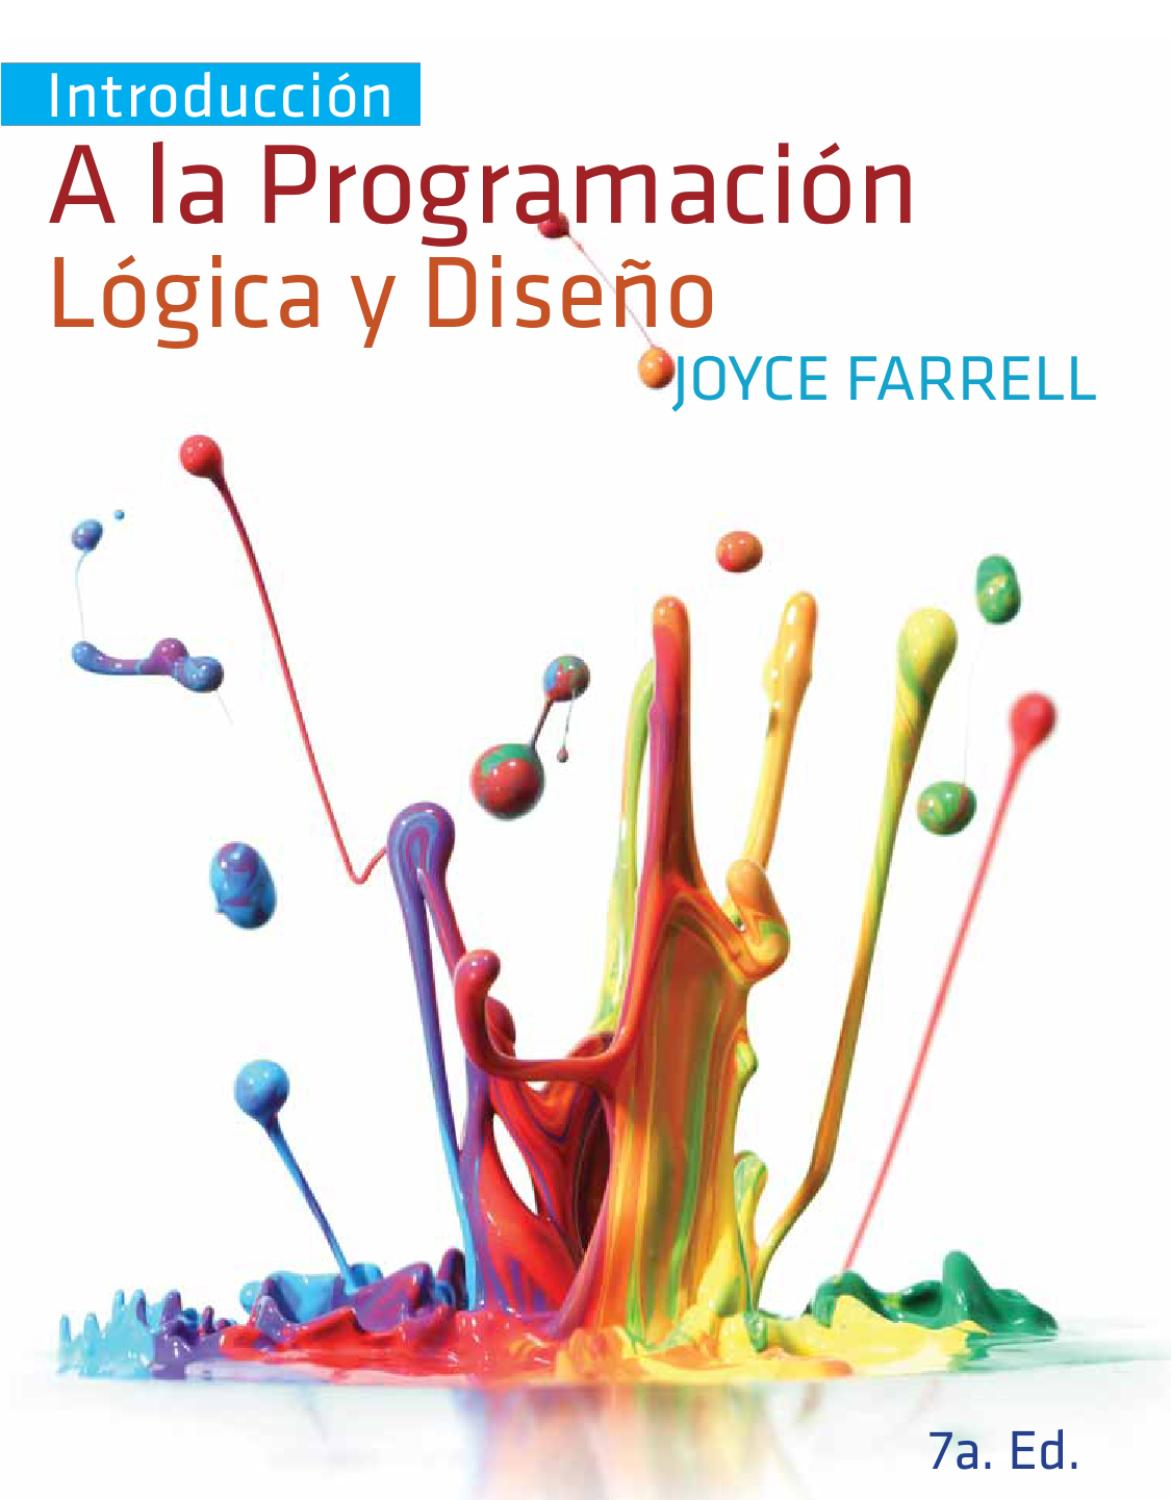
\includegraphics[scale=0.3]{imgs/farrell.jpg}
%       \caption{Libro Guía.}
%     \end{figure}
%   \end{column}
% \end{columns}

% \end{frame}

% \begin{frame}
% \frametitle{Porqué es importante saber programar? www.code.org}
% \begin{figure}[ht]
%   \centering
%   \includegraphics[scale=0.35]{imgs/todoelmundoaprogramar.png}
%   \caption{https://youtu.be/X5Wkp1gsNik}
% \end{figure}
% \end{frame}

% \begin{frame}
% \frametitle{Khan Academy -- Computer Programming}
% \begin{figure}[ht]
%   \centering
%   \includegraphics[scale=0.15]{imgs/khan.png}
%   \caption{https://www.khanacademy.org/computing/computer-programming}
% \end{figure}
% \end{frame}


% %--------------------------------------------------------------------------
% \section{Módulo 1 -- Clase Número 1}
% % Objetivos del Modulo
% % Tiempo a invertir
% \begin{frame}[fragile, shrink=10]
% \frametitle{Objetivos del Módulo}
% El estudiante al concluir este módulo podrá:
% \begin{itemize}
% \item Explicar el proceso global de solución de un problema mediante la programación
% \item Estará capacitado para analizar un problema simple construyendo un modelo con los elementos que intervienen en el problema.
% \item Habrá desarrollado la lógica para la solución de problemas a través de la computadora mediante la representación de algoritmos.
% \item Podrá determinar la secuencia de pasos para dar la solución a un problema, através de la elaboración de \alert{algoritmos}, utilizando \alert{estructura de control} y \alert{estructuras de datos} cada vez más complejas.
% \end{itemize}

% \textbf{Tiempo requerido:} 15 horas de clase y 32 horas de trabajo independiente.
% \end{frame}

% % %% Historia
% \subsection{Historia}
% \begin{frame}
%   \frametitle{Historia}
%   \begin{itemize}
%   \item La computación es una ciencia nueva
%   \item El primer computador comercial es de 1946
%   \item Esto implica que es una ciencia en construcción
%   \item SOMOS PARTE DE ESA HISTORIA
%   \end{itemize}
% \end{frame}

% \begin{frame}
%   \frametitle{Historia}
%   \begin{itemize}
%   \item Los sistemas computacionales actuales son el resultado de los esfuerzos de muchas personas.
%   \item Conocer la historia nos permite valorar lo que tenemos actualmente.
%   \end{itemize}
% \end{frame}

% % \begin{frame}
% %   \frametitle{Algunos eventos clave}
% %   \begin{itemize}
% %   \item Muhammad ibn Musa Al\' Khowarizmi
% %   \item Regla de Cálculo -- 1612
% %   \item Telar automático con tarjetas perforadas -- 1800's
% %   \item Charles Babbage -- 1800's
% %   \item Ada Augusta King
% %   \item Censo de 1890
% %   \item Alan Turing
% %   \item Grace Murray Hopper
% %   \item Eniac -- 1946
% %   \item Transistor
% %   \item Memoria de Núcleos Magnéticos -- 1951
% %   \item Memoria de Tambor -- 1954
% %   \item Lenguaje de programación Fortran -- 1957
% %   \item IBM System/360
% %   \item Sistema Operativo Unix -- 1969
% %   \item Bill Gates, Steve Jobs \& Steve Wozniak
% %   \item PC Seleccionado ``Hombre del año'' por Time en 1982
% %   \item Internet
% %   \item Dispositivos Móviles
% %   \end{itemize}
% % \end{frame}

% \subsection{Definición de Sistema}
% \begin{frame}
%   \frametitle{Qué es un sistema?}
%   \begin{tcolorbox}[colback=blue!5,colframe=blue!40!black,title=Un sistema es...]
%     Una colección intencional de componentes interrelacionados, de diferentes tipos, que trabajan juntos para lograr un objetivo.

% \textbf{Ejemplos:} Sistemas de computador, sistemas operativos, sistemas de pago, sistema de educación, sistema de gobierno, sistema vial, etc.
%   \end{tcolorbox}
% \end{frame}

% \begin{frame}
%   \frametitle{Características de un sistema}
%   \begin{itemize}
%   \item Un sistema puede incluir hardware, software, componentes eléctricos, electrónicos y ser manejado por personas.
%   \item Los componentes del sistema \alert{dependen} de otros componentes del sistema.
%   \item Las propiedades y el comportamiento de los componentes del sistema están \textbf{obligatoriamente} entremezclados.
%   \end{itemize}
% \end{frame}

% \subsection{Hardware y Software}
% %% Hardware y software
% \begin{frame}
%   \frametitle{Hardware y Software}
% Como en la anterior definición. Un sistema de cómputo también es un conjunto de \textbf{elementos electrónicos} que interactúan entre sí, \textit{operando sobre información}

% \begin{itemize}
% \item \textbf{Hardware:} Son los componentes físicos.
% \item \textbf{Software:} Los componentes lógicos e intangibles que indican al hardware las tareas que debe ejecutar.
% \end{itemize}
% \end{frame}

% \begin{frame}
%   \frametitle{John von Neumann}
%   \begin{columns}
%     \begin{column}[ht]{5cm}
%       \begin{itemize}
%       \item Húngaro--Americano
%       \item 1903--1957
%       \item Matemático, Físico, Inventor.
%       \item Proyecto Manhattan. 
%       \item Aportes en áreas como, matemáticas, análisis funcional, geometría, topología, criptografía, mecánica cuántica, hidrodinámica, computación, economía. 
%       \end{itemize}
%     \end{column}
%     \begin{column}[ht]{5cm}
%       \begin{figure}[ht]
%         \centering
%         \includegraphics[scale=0.5]{imgs/neumann.jpg}
%         \caption{\textbf{Tomado de:} Jon von Neumann}
%       \end{figure}
%     \end{column}
%   \end{columns} 
% \end{frame}

% \begin{frame}
%   \frametitle{Hardware: Arquitectura Von Neumann}
%     \begin{figure}[ht]
%       \centering
%       \includegraphics[scale=0.5]{imgs/von.png}
%       \caption{Arquitectura Von Neumann}
%     \end{figure}
% \end{frame}

% \begin{frame}
%   \frametitle{Hardware: Arquitectura Von Neumann}
%     \begin{figure}[ht]
%       \centering
%       \includegraphics[scale=0.1]{imgs/bus.png}
%       \caption{Arquitectura Von Neumann: Bus}
%     \end{figure}
% \end{frame}

% \begin{frame}
%   \frametitle{BUS, MEM, CPU y E/S}
%   \begin{itemize}
%   \item \textbf{BUS:} Comúnica varios dispositivos.
%     \begin{itemize}
%     \item Direccionamiento
%     \item Datos
%     \item Control
%     \end{itemize}
%   \item \textbf{CPU:} Ejecuta programas cargados en memoria principal, toma sus instrucciones, las examina y luego las ejecuta.
%     \begin{itemize}
%     \item Direccionar Memoria y perfiféricos (E/S)
%     \item Funciones Matemáticas y Lógicas
%     \end{itemize}
%   \item \textbf{E/S:}
%     \begin{itemize}
%     \item Conexión con el Mundo
%     \end{itemize}
%   \item \textbf{Memoria:} Elementos que permiten almacenar Información
%   \end{itemize}
% \end{frame}

% \begin{frame}
%   \frametitle{La CPU}
%   \begin{columns}
%     \begin{column}[ht]{5cm}
%       \begin{itemize}
%       \item Unidad de Control (U.C.)
%       \item Unidad Aritmético--Lógica (ALU)
%       \item Registros
%         \begin{itemize}
%         \item Contador de Programa (PC)
%         \item Registro de Instrucción
%         \item Registros de propósito general
%         \end{itemize}
%       \end{itemize}
%     \end{column}
%     \begin{column}[ht]{5cm}
%       \begin{figure}[ht]
%         \centering
%         \includegraphics[scale=0.4]{imgs/cpu.jpg}
%         \caption{\textbf{Tomado de:} Intel Corp.}
%       \end{figure}
%     \end{column}
%   \end{columns} 
% \end{frame}

% \begin{frame}
%   \frametitle{Memoria Primaria}
%   \begin{columns}
%     \begin{column}[ht]{5cm}
%       \begin{itemize}
%       \item RAM
%       \item ROM
%       \end{itemize}
%     \end{column}
%     \begin{column}[ht]{5cm}
%       \begin{figure}[ht]
%         \centering
%         \includegraphics[scale=0.5]{imgs/ram.jpg}
%         \caption{\textbf{Tomado de:} cdn.computerhope.com}
%       \end{figure}
%     \end{column}
%   \end{columns} 
% \end{frame}

% \begin{frame}
%   \frametitle{Memoria Secundaria}
%   \begin{columns}
%     \begin{column}[ht]{5cm}
%       \begin{itemize}
%       \item Discos
%       \item PenDrives
%       \item CD/DVD/BlueRay
%       \item Cintas Magnéticas
%       \item DAT/ZIP
%       \end{itemize}
%     \end{column}
%     \begin{column}[ht]{5cm}
%       \begin{figure}[ht]
%         \centering
%         \includegraphics[scale=0.6]{imgs/disk.jpg}
%         \caption{\textbf{Tomado de:} dilshodzaripov.weebly.com}
%       \end{figure}
%     \end{column}
%   \end{columns} 
% \end{frame}

% \begin{frame}
%   \frametitle{Jerarquía de Memoria}
%   \begin{figure}[ht]
%     \centering
%     \includegraphics[scale=0.3]{imgs/memh.jpg}
%     \caption{\textbf{Tomado de:} computerscience.chemeketa.edu}
%   \end{figure}
% \end{frame}

% \begin{frame}
%   \frametitle{Entrada/Salida}
%   \begin{columns}
%     \begin{column}[ht]{5cm}
%       \begin{itemize}
%       \item Entrada
%         \begin{itemize}
%         \item Teclado, Mouse, Micrófono, Scanner, Lector óptico, Joytick, Tarjeta de Red.
%         \end{itemize}
%       \item Salida
%         \begin{itemize}
%         \item Monitor, Impresora, Parlantes, Tarjeta de Red.
%         \end{itemize}
%       \end{itemize}
%     \end{column}
%     \begin{column}[ht]{5cm}
%       \begin{figure}[ht]
%         \centering
%         \includegraphics[scale=0.1]{imgs/peri.jpg}
%         \caption{\textbf{Tomado de:} 1.bp.blogspot.com}
%       \end{figure}
%     \end{column}
%   \end{columns} 
% \end{frame}

% \begin{frame}
%   \frametitle{MainFrames}
%       \begin{figure}[ht]
%         \centering
%         \includegraphics[scale=0.35]{imgs/mainframe.png}
%         \caption{\textbf{Tomado de:} www.concise-course.com}
%       \end{figure}
% \end{frame}

% \begin{frame}
%   \frametitle{Redes de Computadores}
%   \begin{figure}[ht]
%     \centering
%     \includegraphics[scale=0.4]{imgs/net.jpg}
%     \caption{\textbf{Tomado de:} netdna-cdn.com}
%   \end{figure}
% \end{frame}

% \begin{frame}
%   \frametitle{Alternativas a la Arquitectura de Von Neumann}
%   \begin{columns}
%     \begin{column}[ht]{5cm}
%       \begin{itemize}
%       \item El principal cuello de botella: \textit{Cuando la CPU hace una solicitud para leer una palabra de la memoria, la respuesta proviene de unos cuantos chips y el resto no hace nada.}
%       \item Alternativa: Computación Paralela
%       \end{itemize}
%     \end{column}
%     \begin{column}[ht]{5cm}
%       \begin{figure}[ht]
%         \centering
%         \includegraphics[scale=0.2]{imgs/apolo.jpg}
%         \caption{Apolo}
%       \end{figure}
%     \end{column}
%   \end{columns} 
% \end{frame}

% \begin{frame}
%   \frametitle{Supercomputadores}
%   \begin{figure}[ht]
%     \centering
%     \includegraphics[scale=0.3]{imgs/apolo2.jpg}
%     \caption{Supercomputador Apolo}
%   \end{figure}
% \end{frame}

% \begin{frame}
%   \frametitle{Arquitectura del Computador}
%   \begin{figure}[ht]
%     \centering
%     \includegraphics[scale=0.4]{imgs/arch.png}
%     \caption{\textbf{Tomado de:} minnie.tuhs.org}
%   \end{figure}
% \end{frame}

% \begin{frame}
%   \frametitle{Arquitectura del Computador: Capas}
%   \begin{figure}[ht]
%     \centering
%     \includegraphics[scale=0.7]{imgs/layers.png}
%     \caption{\textbf{Tomado de:} wikimedia.org}
%   \end{figure}
% \end{frame}

% \begin{frame}
%   \frametitle{Tipos de Software}
%   \begin{itemize}
%   \item \textbf{Software del sistema:} Es el programa que controla, coordina y gestiona el hardware. Le dice al computador como usar sus propios componentes. La mayor parte de este software viene incluido en el Sistema Operativo.
%   \item \textbf{Software de Programación:} Es el programa usado para crear y ejecutar otros programas.
%   \item \textbf{Software de Aplicación:} Programa usado para trabajar con el computador. Le dice al computador como realizar las tareas que pide el usuario.
%   \end{itemize}
% \end{frame}

% \begin{frame}
%   \frametitle{Software: Sistemas Operativos}
%   \begin{figure}[ht]
%     \centering
%     \includegraphics[scale=0.4]{imgs/os.png}
%     \caption{\textbf{Tomado de:} 1.bp.blogspot.com}
%   \end{figure}
% \end{frame}

% \begin{frame}
%   \frametitle{Software: Sistemas Operativos}
%   \begin{columns}
%     \begin{column}[ht]{5cm}
%       \begin{itemize}
%       \item Algunos Elementos importantes
%         \begin{itemize}
%         \item Kernel
%         \item Device Drivers
%         \item Shell
%         \item Manejador de Ventanas
%         \end{itemize}
%       \end{itemize}
%     \end{column}
%     \begin{column}[ht]{5cm}
%       \begin{figure}[ht]
%         \centering
%         \includegraphics[scale=0.2]{imgs/apolo.jpg}
%         \caption{Apolo}
%       \end{figure}
%     \end{column}
%   \end{columns} 
% \end{frame}


% \begin{frame}
%   \frametitle{Software: Aplicaciones}
%   \begin{columns}
%     \begin{column}[ht]{5cm}
%       \begin{itemize}
%       \item Son los programas que utiliza un usuario final para llevar a cabo una tarea.
%       \item Algunos tipos son:
%         \begin{itemize}
%         \item Oficina
%         \item CAD/CAM
%         \item GIS
%         \item MIS
%         \end{itemize}
%       \end{itemize}
%     \end{column}
%     \begin{column}[ht]{5cm}
%       \begin{figure}[ht]
%         \centering
%         \includegraphics[scale=0.2]{imgs/apps.jpg}
%         \caption{Mobile Apps}
%       \end{figure}
%     \end{column}
%   \end{columns} 
% \end{frame}

% \begin{frame}
%   \frametitle{Software: Herramientas de Desarrollo}
%   \begin{columns}
%     \begin{column}[ht]{5cm}
%       \begin{itemize}
%       \item Son los programas que utiliza un desarrollador para crear programas.
%       \item Algunas herramientas son:
%         \begin{itemize}
%         \item CASE
%         \item Compiladores
%         \item Depuradores
%         \item Editores
%         \item Gestión de Versiones
%         \item Generadores de Perfiles
%         \item etc, etc...
%         \end{itemize}
%       \end{itemize}
%     \end{column}
%     \begin{column}[ht]{5cm}
%       \begin{figure}[ht]
%         \centering
%         \includegraphics[scale=0.3]{imgs/langs.jpg}
%         \caption{Distintos lenguajes de programación}
%       \end{figure}
%     \end{column}
%   \end{columns} 
% \end{frame}

% \begin{frame}
%   \frametitle{Direcciones, Instrucciones y Datos}
%   \begin{columns}
%     \begin{column}[ht]{5cm}
%       \begin{itemize}
%       \item Un computador solo almacena 1 y 0
%       \item Se requiere de códigos para representar valores diferentes a enteros.
%       \end{itemize}
%     \end{column}
%     \begin{column}[ht]{5cm}
%       \begin{figure}[ht]
%         \centering
%         \includegraphics[scale=0.25]{imgs/ascii.png}
%         \caption{Código ASCII}
%       \end{figure}
%     \end{column}
%   \end{columns} 
% \end{frame}

% \begin{frame}
%   \frametitle{Conversión entre sistemas}
%   \begin{columns}
%     \begin{column}[ht]{5cm}
%       \begin{itemize}
%       \item Sistemas de numeración con otras bases: Horas
%       \item En informática se trabaja en binario, octal y hexadecimal.
%       \end{itemize}
%     \end{column}
%     \begin{column}[ht]{5cm}
%       \begin{figure}[ht]
%         \centering
%         \includegraphics[scale=0.25]{imgs/ascii.png}
%         \caption{Código ASCII}
%       \end{figure}
%     \end{column}
%   \end{columns} 
% \end{frame}

% \begin{frame}
%   \frametitle{Entrada -- Proceso -- Salida}
%   \begin{itemize}
%   \item \textbf{Entrada:} Información que ingresa al sistema para ser procesada o ser parte del proceso.
%   \item \textbf{Procesamiento:} ``Operaciones'' que transforman la entrada en la salida.
%   \item \textbf{Salida:} El resultado de aquello que fue ejecutado.
%   \end{itemize}
% \textbf{Nota:} Puede haber almacenamiento de información y puede haber retroalimentación.
% \end{frame}

% \begin{frame}
%   \frametitle{Entrada -- Proceso -- Salida}
%   \begin{figure}[ht]
%     \centering
%     \includegraphics[scale=0.7]{imgs/process.jpg}
%     \caption{Procesamiento de Información}
%   \end{figure}
% \end{frame}

% \subsection{Algoritmos, lenguajes y programas}

% \begin{frame}[fragile, shrink=10]
%   \frametitle{Qué es un algoritmo?}
%   \begin{tcolorbox}[colback=blue!5,colframe=blue!40!black,title=Un algoritmo es...]
%     una secuencia de instrucciones que representan un modelo de solución para determinado tipo de problemas. O bien como un conjunto de instrucciones que realizadas en orden conducen a obtener la solución de un problema.
%   \end{tcolorbox}
% \end{frame}

% \begin{frame}
%   \frametitle{Qué es un algoritmo?}
%   \begin{tcolorbox}[colback=blue!5,colframe=blue!40!black,title=Un algoritmo es...]
%     un conjunto prescrito de instrucciones o reglas \textbf{bien definidas}, \textbf{ordenadas} y \textbf{finitas} que permite realizar una actividad mediante pasos sucesivos que no generen dudas a quien daba realizar dicha actividad.
%     \begin{flushright}
%       Wikipedia. Algoritmo.
%     \end{flushright}
%   \end{tcolorbox}
% \end{frame}

% \begin{frame}
%   \frametitle{Qué es un algoritmo?}
% \begin{columns}
%   \begin{column}[ht]{5cm}
%     \begin{center}
% ``En la ciencias de la computación, y en la programación, los algoritmos son más importantes que los lenguajes de programación o las computadoras. Un lenguaje de programación es sólo un medio para expresar un algoritmo y una computadora es sólo un procesador para ejecutarlo''      
%     \end{center}
%     \begin{flushleft}
%       \tiny{Luis Joyanes Aguilar. Reconocido Autor de Computación.}
%     \end{flushleft}
%   \end{column}
%   \begin{column}[ht]{5cm}
%     \begin{figure}[ht]
%       \centering
%       \includegraphics[scale=0.5]{imgs/joyanes.jpg}
%       \caption{Luis Joyanes Aguilar}
%     \end{figure}
%   \end{column}
% \end{columns}
% \end{frame}

% \begin{frame}
%   \frametitle{Características de los Algoritmos}
%   \begin{itemize}
%   \item \textbf{Preciso:} Debe definirse de manera rigurosa, sin dar lugar a ambigüedades.
%   \item \textbf{Definido:} Si se sigue un algorimto dos veces, se obtendrá el mismo resultado.
%   \item \textbf{Finito:} Debe terminar en algun momento.
%   \item \textbf{Entrada:} Puede tener cero o más elementos de entrada.
%   \item \textbf{Resultado:} Debe producir un resultado. Los datos de salida serán los resultados de efectuar las instrucciones.
%   \end{itemize}
%   \begin{center}
% Entre dos algoritmos que lleven al mismo objetivo, siempre será preferible el más eficiente. Podría ser el más corto o no. Se deben analizar tiempos de ejecución y recursos.
%   \end{center}
% \end{frame}

% \begin{frame}
%   \frametitle{Diagramas de Flujo}
%     \begin{figure}[ht]
%       \centering
%       \includegraphics[scale=0.33]{imgs/flow.png}
%       \caption{Diagrama de flujo del funcionamiento de una lámpara. De LampFlowchart.svg: svg by Booyabazookaoriginal png by Wapcapletderivative work: Huhsunqu (talk) - LampFlowchart.svg, CC BY-SA 3.0.}
%     \end{figure}
% \end{frame}

% \begin{frame}
%   \frametitle{Diagramas de Flujo}
%     \begin{figure}[ht]
%       \centering
%       \includegraphics[scale=0.5]{imgs/raiz.png}
%       \caption{Diagrama de flujo del algoritmo bailónico para obtener una raíz cuadrada.}
%     \end{figure}
% \end{frame}

% \begin{frame}
%   \frametitle{Qué es el software?}
%   \begin{tcolorbox}[colback=blue!5,colframe=blue!40!black,title=Definición según el estándar 729 IEEE]
%     Es el conjunto de los \textbf{programas de cómputo, procedimientos, reglas, documentación y datos asociados} que forman parte de las operaciones de un sistema de computación.
%   \end{tcolorbox}
% \end{frame}

% \begin{frame}
%   \frametitle{Qué es un lenguaje de programación?}
%   \begin{tcolorbox}[colback=blue!5,colframe=blue!40!black,title=Un lenguaje de programación es...]
%     \begin{itemize}
%     \item Es un sistema \textbf{notacional} para describir computaciones en una forma legible tanto para la máquina como para el ser humano.
%     \item Es un \textbf{lenguaje formal} y/o \textbf{estructurado} (reglas semánticas y sintácticas) para expresar \textbf{procesos} y/o \textbf{comportamientos físicos y lógicos} que pueden ser ejecutados por computadoras.
%     \end{itemize}
%   \end{tcolorbox}
% \end{frame}

% \begin{frame}
%   \frametitle{Niveles de los lenguajes de programación}
%   \begin{tcolorbox}[colback=blue!5,colframe=blue!40!black,title=Lenguaje de máquina]
%     Es el sistema de códigos directamente interpretable por un circuito.
%   \end{tcolorbox}
% \end{frame}

% \begin{frame}
%   \frametitle{Niveles de los lenguajes de programación}
%   \begin{tcolorbox}[colback=blue!5,colframe=blue!40!black,title=Lenguaje Ensamblador]
%     Implementa una representación simbólica de los códigos de máquina binarios y otras constantes, este es la representación más directa del código de máquina especificado por cada arquitectura.
%   \end{tcolorbox}
% \end{frame}

% \begin{frame}
%   \frametitle{Niveles de los lenguajes de programación}
%   \begin{tcolorbox}[colback=blue!5,colframe=blue!40!black,title=Lenguaje de alto nivel]
%     De un nivel más alto de abstracción que el lenguaje de máquina. Expresa algoritmos de una manera adecuada a la capacidad cognitiva humana.
%   \end{tcolorbox}
% \end{frame}

% \begin{frame}
%   \frametitle{Interpretación y Compilación}
%   \begin{itemize}
%   \item \textbf{Lenguajes Interpretados:} Están destinados a ser ejecutados utilizando un intérprete. O sea, sus instrucciones se \textbf{interpretan} una a una en tiempo de ejecución a un lenguaje intermedio a lenguaje de máquina o a través de una máquina virtual.
%   \item \textbf{Lenguajes Compilados:} Son lenguajes que utilizan un compilador, o sea, éste se \textbf{traduce} a partir de su código fuente por medio de un compilador, en un archivo ejecutable para una determinada plataforma.
%   \end{itemize}
% \end{frame}

% \begin{frame}
%   \frametitle{Ciclo de desarrollo del programa}
%   \begin{itemize}
%   \item Entender el problema
%   \item Planear la lógica
%   \item Codificar el sistema
%   \item Usar software (un compilador o intérprete) para traducir el programa a lenguaje de máquina
%   \item Probar el programa
%   \item Poner el programa en producción
%   \item Mantener el programa
%   \end{itemize}
% \end{frame}

% \begin{frame}
%   \frametitle{Ciclo de desarrollo del programa}
%   \begin{itemize}
%   \item \textbf{Seudocódigo:} Es el uso de convenciones estructurales de los lenguajes pero de una forma ``informal''.
%   \item \textbf{Diagrama de flujo:} Representación gráfica de un proceso o de un algoritmo.
%   \item \textbf{Ambiente de Desarrollo:} También conocido como \textit{Integrated Development Environment} (IDE) en inglés, es un software que ofrece los servicios integrales de editor, depurador, compilador y/o intérprete para el desarrollo de software.
%   \end{itemize}
% \end{frame}

% \begin{frame}
% \frametitle{Primer Ejercicio en PSeInt}
% \begin{itemize}
% \item Descubra el IDE de PSeInt
% \item Busque la ayuda de PSeInt
% \item Realizar el ``hola mundo'' en PSeInt. 
% \item Ejecute el ejemplo \texttt{Suma.psc} que trae la herramienta y al menos otros dos ejemplos.
% \end{itemize}
% \end{frame}

% \begin{frame}
% \frametitle{Documental -- Código Linux}
% \begin{figure}[ht]
%   \centering
%   \includegraphics[scale=0.35]{imgs/linux.jpg}
%   \caption{https://youtu.be/cwptTf-64Uo}
% \end{figure}
% \end{frame}

% \subsection{Tarea}
% \begin{frame}[fragile,shrink=10]
% \frametitle{Tarea}
% \begin{columns}
%   \begin{column}[ht]{5cm}
%     \begin{itemize}
%       \item Por cada hora de clase son tres horas de trabajo por fuera del aula
%       \item Bajar e instalar la herramienta PSeInt. http://pseint.sourceforge.net/
%       \item Ejecute al menos otros dos ejemplos de PSeInt y trate de entenderlos. Traiga preguntas a clase.
%       \item Leer el primer capítulo del libro y realizar los ejercicios.
%       \item Ver Código Linux, para discutir la próxima clase.
%     \end{itemize}
%   \end{column}
%   \begin{column}[ht]{5cm}
%     \begin{figure}[ht]
%       \centering
%       \includegraphics[scale=0.23]{imgs/tarea1.png}
%       \caption{PSeInt}
%     \end{figure}
%   \end{column}
% \end{columns}
% \end{frame}

% \begin{frame}
%   \frametitle{Tarea}
%   \begin{itemize}
%   \item Leer y entender los diagramas de flujo.
%   \item Lectura del capítulo 2.
%   \item Crear un programa simple que esté en el libro en PSeInt por medio de los diagramas de flujo que esta herramienta presenta.
%   \end{itemize}
% \end{frame}

% \begin{frame}
%   \frametitle{Referencias}
%   \begin{itemize}
%   \item Joyce Farrell. Introducción a la programación lógica y diseño.
%   \item Notas de clase. J.F. Cardona, Universidad EAFIT.
%   \item Notas de clase. E. Suescún, Universidad EAFIT.
%   \item Notas de clase. J.G. Lalinde, Universidad EAFIT.
%   \end{itemize}
% \end{frame}
\end{document}
